\documentclass{article}
\usepackage[utf8]{inputenc}
\usepackage{graphicx}
\usepackage[T1]{fontenc}
\usepackage{lmodern}
\usepackage{hyperref}
\usepackage{xcolor}
\usepackage{booktabs}

\title{pi-lab}
\date{October 2020}

\newcommand{\resource}[1]{(Local copy saved to \texttt{#1})}
\newcommand{\tttilde}[0]{\textasciitilde{}}
\newcommand{\todo}[1]{{\color{blue}{TODO: #1}}}

\begin{document}

\title{Assignment 1}

\section{Background}

\subsection{Cluster architecture}

This document provides instructions for building a cluster computer which uses three Raspberry Pi microcomputers. Each physical computer comprising the cluster is called a \emph{node} of the cluster; here, each Raspberry Pi will be a node.

In order for a cluster computer to be effective, its nodes must be able to communicate efficiently. The cluster nodes here will communicate via Ethernet connections between the nodes and a network switch. In addition to using the switch to physically connect the cluster, one of the nodes will act as a \emph{router} for the cluster after installing \emph{DHCP server} software. This will automatically assign IP addresses to the other non-router nodes in the cluster when they are connected, serving the same purpose that wireless routers often do in home Wi-Fi networks. The DHCP server software is very light, so the router node will still be acting as a regular cluster node as well with essentially no drop in performance. 

In order to use the cluster, one needs a way of communicating with (and executing commands on) its nodes. This will be done by establishing an \emph{SSH connection} from a desktop or laptop computer to each cluster node, which allows one to remotely run programs on the cluster. The SSH connection will be made over a Wi-Fi network, which can either be one's home network or a mobile hotspot network created with a smartphone's data connection.

The following diagram summarizes the architecture described above.

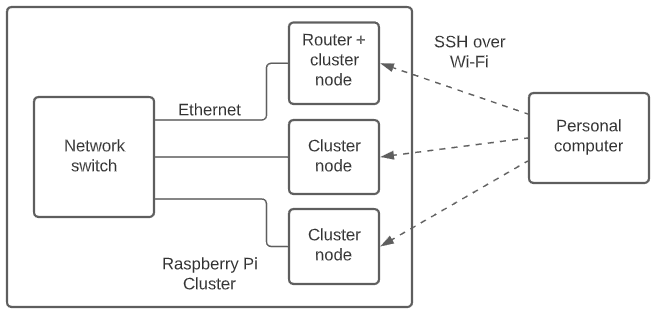
\includegraphics[width=\textwidth]{images/cluster-diagram.png}

\subsection{Cluster benchmarking}

To get a sense of how the cluster computer's performance scales with the amount of processor power being used, the benchmarking program HPL (High-Performance Linpack) will be used. HPL creates and solves a system of linear equations, the size of which can be arbitrarily scaled to best fit the size and power of the system being tested. HPL is designed for benchmarking distributed systems, so it will automatically split the computation up efficiently between the nodes of the system.

HPL relies on two other software tools: an MPI library (Message Passing Interface) to communicate between nodes, and a BLAS library (Basic Linear Algebra Subprograms) to run atomic floating-point operations that are optimized for the node's architecture. In this lab, MPICH and OpenBLAS will be used. Both will need to be built from source on each node in the cluster, since a prebuilt executable is unavailable for the Raspberry Pi architecture.

\section{Component lists}

\subsection{Universal items}
These items will be needed for any configuration of Raspberry Pi cluster. The list is designed for a 3-node cluster, but can be scaled accordingly for a cluster of any size. 

In addition to the components in this section, you will need to choose a configuration given in a later section to build a complete cluster.

\begin{itemize}
    \item \textbf{3x Raspberry Pi 4B} (2GB RAM)
    
    Note that the Raspberry Pi 4B is available with 2GB, 4GB, and 8GB memory. The models with more RAM are useful when using a Pi as a desktop computer, but higher RAM will not meaningfully improve the cluster's performance for our purposes, so the cheapest model is sufficient for this lab.
    
    The previous Raspberry Pi model 3B+ is priced similarly to the 4B with 2GB RAM. However, the 4B comes equipped with Gigabit Ethernet capability (up to 950Mbps bandwidth in practice), while the 3B+ only emulates it via Gigabit Ethernet over USB, which has a significantly lower peak bandwidth (under 300Mbps). Since our cluster nodes will communicate over an Ethernet connection, its bandwidth is an important bottleneck for the speed of the cluster, and hence the model 4B is preferable over 3B+.
        
    \item \textbf{3x Ethernet Cat6 cables}
    
    These cables will connect the Pi to the Ethernet switch. It can be convenient for these cables to be on the short side (even $1$ft should be enough).
    
    \item \textbf{3x 16GB Micro SD cards}
    
    Each Pi will need its own micro SD card, which will contain its operating system. SD cards with more memory will also work.
    
    \item \textbf{Micro SD to USB adapter}
    
    This item is used to connect a Micro SD card to a computer, which will be necessary to write the Raspberry Pi operating system. Any means of accessing a Micro SD card from a computer will work (such as a slot in the computer itself).
    
    \item \textbf{3x Raspberry Pi cases} (optional)
    
    Note that using PoE HATs will increase the height of each Pi, causing some cases not to fit. Also, cases with no ventilation will probably cause significantly higher temperatures, ultimately hurting performance.
    
\end{itemize}

\subsection{3-node cluster using PoE}

This cluster configuration will use PoE (Power over Ethernet) to power each node. Specifically, the network switch that allows the cluster to communicate over Ethernet will also be providing power to the cluster. The benefit of this is a simplified physical cluster layout with fewer cables, since no power-specific cables are needed. The downside is a higher cost of the components.

\begin{itemize}
    \item \textbf{3x PoE HAT}
        
    The PoE HAT is an attachment for the Raspberry Pi 3B+ and 4B that lets the Pi draw power from an Ethernet cable. It also provides a cooling fan, which automatically activates when the temperature of the Pi increases beyond a certain threshold.
    
    \item \textbf{TP-LINK TL-SG1005P Ethernet switch}
    
    This Gigabit Ethernet switch is compatible with PoE and will provide enough power to run $3$ Raspberry Pi 4B nodes simultaneously, assuming each Pi has a PoE HAT.
\end{itemize}

\subsection{3-node cluster using USB-C power}

In this configuration, power is supplied to each Pi through the official USB-C power supply cable. Because of this, the network switch need not be compatible with PoE, and so a less expensive model can be used compared to the PoE switch. configuration.

\begin{itemize}
    \item \textbf{3x Official Raspberry Pi 15.3W USB-C Power Supply}
    
    \item \textbf{TP-LINK TL-SG1005D Ethernet switch}
    
    This switch does not have PoE compatibility so it can't be used with the PoE cluster configuration. This is reflected in its lower price compared to the switch.
\end{itemize}

\section{Hardware setup}

\subsection{Wi-Fi network}

The purpose of this section is to set up a Wi-Fi network where one has access to the list of devices connected to the network. This is easier to accomplish at home, where one has admin-level access to a wireless router, but can also be accomplished with a mobile hotspot network created by a smartphone. Both options are presented below, and only one set of instructions needs to be followed. Using a home network is preferable, since no mobile data will be used.

Regardless of the source of the Wi-Fi network being used, record the SSID (network name) and password of the network, which will be needed later.

\subsubsection{Using a wireless home network}
\begin{itemize}
    \item Connect to your router in a web browser by entering the router's IP address in the address bar. The router's IP address will vary depending on your ISP, so you will need to Google it if you don't already know what it is. Below is a screenshot of the Xfinity router admin panel login screen, which can be reached at IP address \texttt{10.0.0.1}.
    
    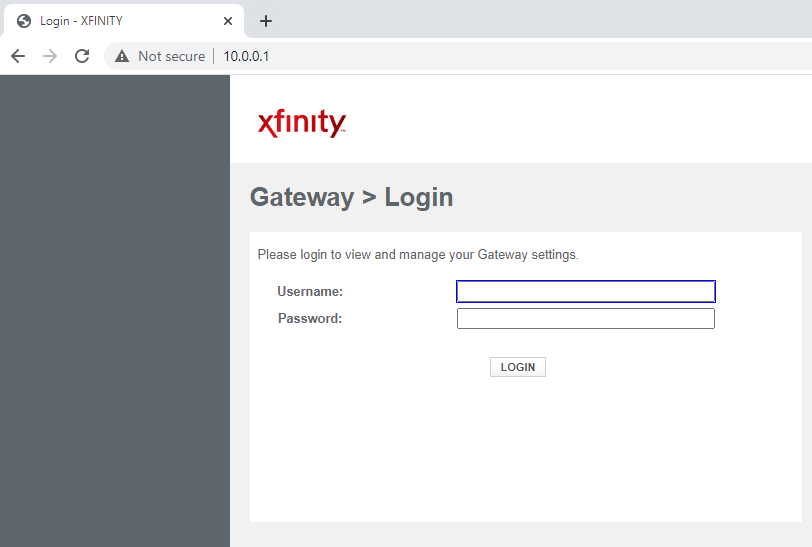
\includegraphics[width=\textwidth]{images/router-panel.png}
    
    \item You will also need to know the username and password of your router to access its admin panel. The default login information for your router can be looked up on Google. As an example, the default username and password on an Xfinity router are \texttt{admin} and \texttt{password}, respectively.
    
    \textbf{Note:} You might want to take this opportunity to change your router's password from its default if you haven't already.
    
    \item Once logged into the router's admin panel, note how to view the list of devices connected to the router, which should list the IP address of each device on the router's wireless network.
\end{itemize}
	
\subsubsection{Using a mobile hotspot network}
\begin{itemize}
    \item In lieu of a home network where one has admin-level access to a router, a smartphone can be used to generate a mobile hotspot, which is a small Wi-Fi network controlled by the phone.
    
    Setting up a mobile hotspot will be different depending on your phone's operating system, but many resources on how to do so can be found using a Google search. (As an example, on Android phones, "mobile hotspot" should be an option in the pull-down settings menu). 
    
    \item Once a mobile hotspot is created, try connecting to it over Wi-Fi from a computer to make sure that it works.  Note down the network's SSID and password, which will be used later. 
    
    \item While the computer is connected to the mobile hotspot, find the list of connected devices on the smartphone and confirm that the computer appears on the list, which should appear in the same menu used to initiate the mobile hotspot. Use the list to find the computer's IP address on the mobile hotspot network (on Android, tap the device on the connected devices list to see its IP address).
\end{itemize}
	
\subsection{Configure Raspberry Pi OS on a Micro SD card}
\label{sec:configure-os}
In this section, you will write Raspberry Pi OS to a Micro SD Card. The SD card will then be accessed in a terminal to make further adjustments to the default Raspberry Pi OS. Namely, we will enable SSH and enforce automatic connection to a Wi-Fi network, which are both needed to connect to the Pi in a \emph{headless} way (i.e. without ever connecting the Pi to a monitor, mouse, or other peripherals).

\textbf{Note:} Since each cluster node will need the configured Raspberry Pi OS on its own Micro SD card, section \ref{sec:configure-os} will need to be followed as many times as there are nodes in the cluster.

\subsubsection{Use the Raspberry Pi Imager to write the default OS}
\begin{itemize}
    \item Download and install the Raspberry Pi Imager for your computer's operating system from \url{https://www.raspberrypi.org/downloads/}. This is the software that will format an SD card to act as an operating system for a Raspberry Pi.
    
    \item Insert a Micro SD card into your computer. Note that the existing contents of the SD card will be erased to write the Raspberry Pi OS.
    
    \item Open the Raspberry Pi Imager and select the "Raspberry Pi OS (32-bit)" operating system and an inserted SD card.
    
    \item Write the OS. This can take around $10$ to $20$ minutes depending on the speed of your internet connection, since the Imager downloads the OS from the internet before it writes.

    \item The Raspberry Pi Imager may eject the SD card after it finishes installing, so you may need to take the SD card out and reinsert it to continue the following steps.
\end{itemize}

\textbf{Note:} The goal of the next section is to use a terminal to open the SD card on which Raspberry Pi OS was just written. The instructions will depend on your computer's operating system, and you should only follow the steps pertaining to your operating system. 

\subsubsection{Open the SD card in a terminal (MacOS)}
\begin{itemize}
    \item On MacOS (and any other Unix-like OS, like Linux and its variants), the default terminal program can be used. To open it on MacOS, search for \texttt{Terminal} from the Launchpad application listing. 
    
    \item On MacOS, the SD card should appear in the directory \texttt{/Volumes}, so that the path to the SD card directory is \texttt{/Volumes/boot}.
    
    Run the command \texttt{cd /Volumes/boot} to navigate to the SD card's directory from the terminal.
\end{itemize}

\subsubsection{Open the SD card in a terminal (Windows)}
\begin{itemize}
    \item On Windows, a third-party terminal will need to be installed. Download and install Git Bash from \url{https://www.gitforwindows.org}. 
    
    \item If the SD card has had Raspberry Pi OS correctly written, it should appear as a letter drive named \texttt{boot} in the \texttt{This PC} app on Windows 10 (also known as \texttt{My Computer} on older versions of Windows). For example, in the following screenshot the SD card is the D drive:
    
    
\includegraphics[width=\textwidth]{images/windows-boot-drive.png}
    
    \item The path to the SD card will be a forward slash followed by the \emph{lowercase} letter of the \texttt{boot} drive in the previous step. For example, if \texttt{boot} was the D drive, the path will be \texttt{/d}. 
    
    \item From the Git Bash terminal program, run the command \texttt{cd /d} to navigate to the SD card's directory (replacing \texttt{/d} with the correct path found above).
\end{itemize}

\subsubsection{Configure the default OS from a terminal}

\begin{itemize}
    \item From the SD card's directory, use the \texttt{ls} command, which lists the files in the current directory. Confirm that the returned list of files looks like this:
    
    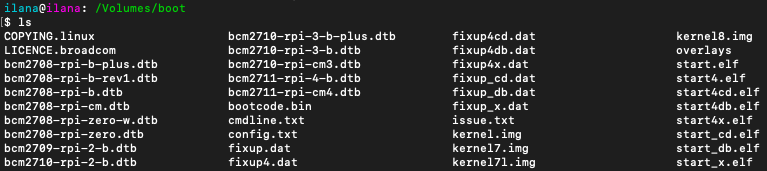
\includegraphics[width=\textwidth]{images/sd-card-ls.png}

    \item Two files need to be added to the \texttt{boot} directory and will be used by the Pi OS during initialization. A blank file can be created in the terminal by using the \texttt{touch} command. 
    
    \item Use the command \texttt{touch ssh} to create a blank file named \texttt{ssh} on the SD card. The presence of the \texttt{ssh} file will enable remote communication with the Pi via SSH. 
    
    \textbf{Note:} SSH can also be enabled by changing a setting in Raspberry Pi OS. However, this setting can't be changed via SSH, since SSH is disabled by default. The benefit of adding the \texttt{ssh} file is that it allows the very first communication with Raspberry Pi OS to be via SSH.
    
    \item Use the \texttt{ls} command again to check that the \texttt{ssh} file now appears in the file list.
    
    \item Run \texttt{touch wpa\_supplicant.conf} to create a blank file named \texttt{wpa\_supplicant.conf}. This file is used to immediately connect the Raspberry Pi to a given Wi-Fi network when it first boots.
    
    \item Run \texttt{nano wpa\_supplicant.conf} to open the \texttt{wpa\_supplicant.conf} file in the Nano text editor, which runs inside the terminal window.
    
    \item Replacing \texttt{SSID} and \texttt{PASSWORD} with your previously chosen SSID and password (and making sure both are still in double quotes), write the following text to the file - make sure the whitespace matches.
\begin{verbatim}
ctrl_interface=DIR=/var/run/wpa_supplicant GROUP=netdev
update_config=1
country=US

network={
  ssid="SSID"
  psk="PASSWORD"
}
\end{verbatim}

\item Save the text (Control+O, then Enter) and close the editor (Control+X).

\item Use the \texttt{cat} command to display the contents of the \texttt{wpa\_supplicant.conf} file and double check it matches the following, except with your chosen network name and password:

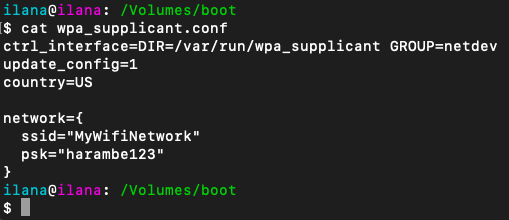
\includegraphics[width=\textwidth]{images/cat-wpa-supplicant.png}

\item The SD card can now be ejected.
\end{itemize}

\subsection{Connect cluster hardware}

In this section, the goal is to put together all of the cluster hardware. Some steps will be different depending on which method you are using to provide power to the cluster.

\begin{itemize}
    \item If using a PoE cluster, attach a PoE HAT to each Raspberry Pi using the provided screws and spacers. 
    
    \item Insert a Micro SD card with the Raspberry Pi OS configured in Section \ref{sec:configure-os} into each Raspberry Pi.
    
    \item Connect each Raspberry Pi to the network switch via an Ethernet cable. 
    
    \item Power on the network switch. (If using a PoE cluster, this will also provide power to each Raspberry Pi.)
    
    \item If using a USB-C powered cluster, plug in a USB cable to each Raspberry Pi. This will power each Pi on.
    
    \item If using a smartphone mobile hotspot as a Wi-Fi network, start it now. Double-check the network's SSID and password match what were previously written on the Pi OS. (If not, it will probably be easier to change the phone to match the SD cards rather than the other way around.)
    
    \item Whether using a mobile hotspot network or a home wireless network, you can confirm that everything is working by the appearance of three new entries in the network's connected devices list. All should be named something similar to \texttt{raspberrypi}, which is the default hostname on Raspberry Pi OS.
    
    \textbf{Note:} if the \texttt{raspberrypi} devices do not appear, it might be necessary to repeat the steps in Section \ref{sec:configure-os} that lead to creating \texttt{wpa\_supplicant.conf}, which is the file that configures the automatic Wi-Fi connectivity. 
\end{itemize}

\section{Install software on cluster nodes}

\subsection{SSH into cluster node}

In this section, you will establish an SSH (Secure Shell) connection to a Raspberry Pi over a Wi-Fi network. An SSH connection allows one to run terminal commands on a remote system; in this case, it allows us to run commands on a computer and have them be executed on a Raspberry Pi.

These steps will be used repeatedly throughout the remainder of the lab to connect to the nodes in the cluster. The phrase "SSH into a cluster node"  refers to following this procedure to establish an SSH connection to that cluster node.

\begin{itemize}
    \item Using the list of connected devices, find the IP address of a \texttt{raspberrypi} device on the hotspot network. If there are multiple connected \texttt{raspberrypi} devices, choose any of their IP addresses.
    
    \item Connect a computer to the same Wi-Fi network (if it isn't already) and open a terminal on the computer.
    
    \item From the computer's terminal, run the command \texttt{ssh pi@IPADDRESS}, replacing \texttt{IPADDRESS} with the previously noted IP address of the Raspberry Pi. The terminal should prompt for a password, which is \texttt{raspberry}. If you are asked if you want to continue connecting, answer \texttt{yes}. 
    
    An example of this prompt is shown in the following screenshot, where the Pi's IP address is \texttt{10.0.0.176}.
    
    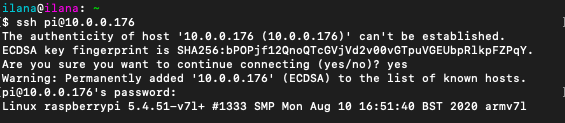
\includegraphics[width=\textwidth]{images/ssh.png}
    
    \textbf{Note:} this step relies on the default username and password values on Raspberry Pi OS, which are \texttt{pi} and \texttt{raspberry}, respectively.
    
    \item Once an SSH connection to the Pi is established in a terminal, commands entered in that terminal will be executed on the Pi.
    
    \item Useful general-purpose commands to know about are:
    \begin{itemize}
        \item \texttt{logout}, which ends the current SSH connection.
        \item \texttt{sudo reboot}, which reboots the Raspberry Pi. This will immediately end the SSH connection.
        \item \texttt{sudo poweroff}, which shuts down the Raspberry Pi. This will also immediately end the SSH connection.
    \end{itemize}
\end{itemize}

\subsection{Give cluster node a unique hostname}
\begin{itemize}
    \item Run \texttt{sudo raspi-config} to open the built-in configuration program for Raspberry Pi OS.
    
    \item Select \texttt{2. Network Options} and then \texttt{N1 Hostname}.
    
    \item Replace the default \texttt{raspberrypi} hostname with something that uniquely identifies this cluster node. You should also distinguish the router by its hostname. In these instructions, the router node will have hostname \texttt{pi-router} and the non-router cluster nodes will be \texttt{pi-node1} and \texttt{pi-node2}.
    
    \textbf{Note:} There's an important distinction between a node's \emph{hostname}, which was just changed, and the \emph{username} used to SSH into a node. The device's hostname effectively identifies the device itself on the network, whereas the username \texttt{pi} is only a user profile recognized by that device's OS.  
    
    \item Exit out of the configuration program, which will prompt you to reboot to save the hostname. Rebooting will automatically close the SSH connection.  
    
    \textbf{Note:} In case you have multiple nodes in the cluster all named \texttt{raspberrypi}, the reboot may be your first opportunity to tell which node just had its hostname changed. You can take this opportunity to physically distinguish the node by its hostname, such as with a sticky note on its Ethernet cable.
    
    \textbf{Note:} The Up arrow can be used to bring back commands that were previous executed in a terminal. This is a quick way to re-establish the same SSH connection without having to retype the command.
\end{itemize}

\subsection{Install software for HPL benchmarks}

This section will need to be completed for each Pi in the cluster, including the Pi being used as a router. Begin by establishing an SSH connection into the Pi on which software will be installed.

\textbf{Note:} When copying shell commands, anything following a \texttt{\#} character on a line is a \emph{comment} and doesn't need to be typed (the comments can be included, but the shell will ignore them).

\subsubsection{Install MPICH}
\begin{itemize}
    \item Run the following shell commands to download and install MPICH:
\begin{verbatim}
# install a Fortran library, which is needed by MPICH
sudo apt update
sudo apt install gfortran

# download the MPICH 3.3 source code to the home directory
wget http://www.mpich.org/static/downloads/3.3/mpich-3.3.tar.gz

# unpack the source code from the TAR archive (similar to a ZIP)
tar xfz mpich-3.3.tar.gz    

# create a directory to hold the MPICH binaries
sudo mkdir -p /home/rpimpi/mpi-install

# create and navigate to a directory to # hold the configured MPICH source
mkdir ~/mpi-build
cd ~/mpi-build

# run the MPICH configure script to build the source
sudo ~/mpich-3.3/configure -prefix=/home/rpimpi/mpi-install

# build the MPICH binaries
# note: this will take around 45 minutes
sudo make
sudo make install    
\end{verbatim}

    \item Verify that the installation was successful by checking the contents of the directories \texttt{/home/rpimpi/mpi-install} and \texttt{/home/rpimpi/mpi-install/bin} match the following screenshot:
    
    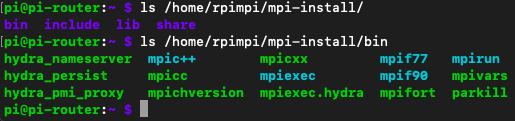
\includegraphics[width=\textwidth]{images/mpi-after-install.png}

    \item Run \texttt{sudo nano \tttilde/.bashrc}, which opens an initialization shell script that runs automatically before every terminal session. Scroll to the bottom and add the following lines:
    
\begin{verbatim}
MPICH_HOME=/home/rpimpi/mpi-install
MPICC=$MPICH_HOME/bin/mpicc
PATH=$PATH:$MPICH_HOME/bin
\end{verbatim}

    \item Save and close \texttt{.bashrc}. 
    
    \item Run the command \texttt{source \tttilde/.bashrc} to re-run the \texttt{.bashrc} script and define the new variables in the current shell. 
    
    \item Check that this worked with the command \texttt{echo \$MPICH\_HOME}, which should output the value that was just added: \texttt{/home/rpimpi/mpi-install}.
    
    \item Also, run the command \texttt{which mpiexec}, which should output the path of the \texttt{mpiexec} program that can now be found in the \texttt{\$PATH}.

\end{itemize}

\subsubsection{Install OpenBLAS}
\begin{itemize}
    \item Run the following shell commands to download and install OpenBLAS.
\begin{verbatim}
# download and unpack the OpenBLAS source code to the home directory
cd
wget http://github.com/xianyi/OpenBLAS/archive/v0.2.20.tar.gz
tar xfz v0.2.20.tar.gz

# make a directory to install the OpenBLAS binaries
mkdir ~/openblas-install

# run the build and install scripts included with the source code
# this may take up to 20 minutes
cd ~/OpenBLAS-0.2.20
sudo make
sudo make install PREFIX=~/openblas-install
\end{verbatim}    

    \item Verify that the installation was successful by checking the contents of the directories as in the following screenshot:
    
    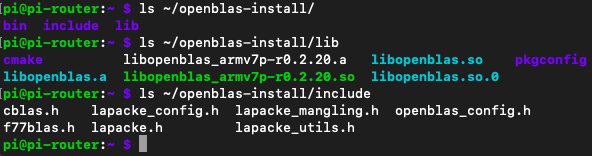
\includegraphics[width=\textwidth]{images/openblas-after-install.png}
\end{itemize}

\subsubsection{Install HPL}
\begin{itemize}
    \item Run the following shell commands to download and prepare HPL for installation:
    
\begin{verbatim}
# download and unpack the HPL source code to the home directory
cd
wget http://www.netlib.org/benchmark/hpl/hpl-2.3.tar.gz
tar xfz hpl-2.3.tar.gz

# generate a generic Makefile for Raspberry Pi OS 
# running make_generic will create the file Make.UNKNOWN
cd hpl-2.3/setup
sh make_generic

# copy the created Makefile into the root HPL directory,
# and name the file extension .rpi for Raspberry Pi
cp Make.UNKNOWN ../Make.rpi

# open the created Makefile in a text editor
cd ..
nano Make.rpi
\end{verbatim}   

    \item The \texttt{Make.rpi} script defines various environment variables needed to build and run HPL. In particular, the script needs to know the directories where MPICH and OpenBLAS were installed (these are the variables \texttt{MPdir} and \texttt{LAdir}, respectively).
    
    Change the following variable definitions in \texttt{Make.rpi} so that they match what's listed below. They are listed here in the same order as they appear in \texttt{Make.rpi}. If a variable in \texttt{Make.rpi} doesn't appear below, its value is correct and doesn't need to be changed.
\begin{verbatim}
ARCH = rpi

TOPdir = $(HOME)/hpl-2.3

MPdir = /home/rpimpi/mpi-install
MPinc = -I $(MPdir)/include
MPlib = $(MPdir)/lib/libmpich.so

LAdir = /home/pi/openblas-install
LAinc = $(LAdir)/include
LAlib = $(LAdir)/lib/libopenblas.so
\end{verbatim}  

    \item Save and close the file once all the above values have been adjusted.

    \item Run \texttt{make arch=rpi} to build HPL using the new values in \texttt{Make.rpi}.
    
    \item Verify that the installation was successful by checking the contents of \texttt{bin/rpi}:
    
    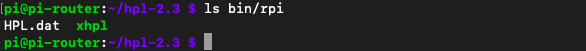
\includegraphics[width=\textwidth]{images/hpl-after-building.png}
\end{itemize}

\subsection{Install and configure router software}

This section will install the software needed to configure a Raspberry Pi as a router for the cluster. Only one node with this software installed is needed, regardless of the number of nodes in the cluster, so this section should only be completed once.

\subsubsection{Configure \texttt{dhcpcd}}

\texttt{dhcpcd} is a DHCP client (not server) that is installed by default on each of the cluster nodes. The presence of \texttt{dhcpcd} on non-router cluster nodes is why they will automatically connect with the DHCP server that will be installed on the router node. On the router node, the \texttt{dhcpcd.conf} configure

\begin{itemize}
    \item Run \texttt{sudo nano /etc/dhcpcd.conf} to open the \texttt{dhcpcd} configuration file in a text editor.
    
    \item Scroll down to the bottom of the file and add the following four lines text at the end:
\begin{verbatim}
interface eth0
static ip_address=192.168.100.1/8
static domain_name_servers=8.8.8.8,8.8.4.4
\end{verbatim}
    
    \item Save and close the file. 
\end{itemize}
    
    Note: the Ethernet port on a Pi is known to the operating system as \texttt{eth0}, so the first line identifies this network interface as the one being modified. The lines establish a static IP address of \texttt{192.168.100.1} for this Pi (in other words, the IP address will always be \texttt{192.168.100.1}) so that the other nodes in the cluster will know a consistent address for their router.

\subsubsection{Install and configure \texttt{dnsmasq}}

\begin{itemize}
    \item Run \texttt{sudo apt install dnsmasq} to install \texttt{dnsmasq} on the router node. \texttt{dnsmasq} is the DHCP server software that the router will use.
    
    \item Run \texttt{sudo rm /etc/dnsmasq.conf} to delete the default \texttt{dnsmasq} configuration file.
    
    \item Run \texttt{sudo nano /etc/dnsmasq.conf} and write the following text into the blank configuration file. Save and close the file when finished.

\begin{verbatim}
interface=eth0
listen-address=192.168.100.1
dhcp-range=192.168.100.32,192.168.100.128,12h
server=8.8.8.8
server=8.8.4.4
domain-needed
bogus-priv
expand-hosts
\end{verbatim}    

    \item Run \texttt{sudo nano /etc/init.d/dnsmasq} to open the initialization script for \texttt{dnsmasq}. Immediately underneath the first line (which should be \texttt{\#!/bin/sh}), add the line \texttt{sleep 10}. The file should look like the following:
    
    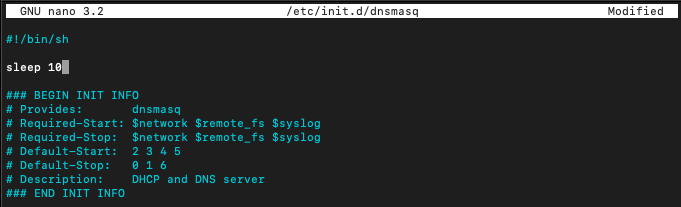
\includegraphics[width=\textwidth]{images/dnsmasq-sleep.png}
    
    \item Save and close the \texttt{/etc/init.d/dnsmasq} file.
    
    \item Run \texttt{sudo reboot} to reboot the Pi. This will automatically break the SSH connection.
    
    \item Wait about a minute for the reboot, then reestablish the SSH connection to the Pi.
    
    \item Run \texttt{sudo service dnsmasq status} on the router node to check that \texttt{dnsmasq} was correctly installed. Make sure that the green text \texttt{Active: active (running)} appears, as in the fourth line of the following image:
    
    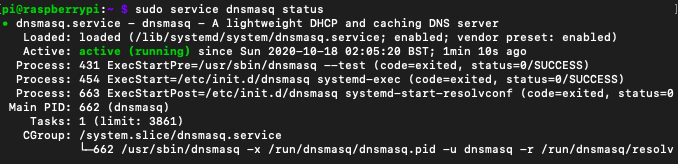
\includegraphics[width=\textwidth]{images/dnsmasq-status.png}
    
    \item Confirm the successful connection of each non-router node to the DHCP server on the router node with the command \texttt{cat /var/lib/misc/dnsmasq.leases}, as shown in the following screenshot:

    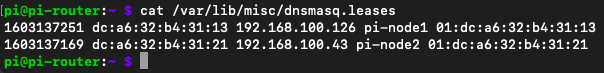
\includegraphics[width=\textwidth]{images/dnsmasq-leases.png}
    
    \item Each non-router node should have an entry line in the above listing. Record the IP addresses of each node, which will be needed later. In the above screenshot, \texttt{pi-node1} has IP address \texttt{192.168.100.126} and \texttt{pi-node2} has IP address \texttt{192.168.100.43}.
    
    \textbf{Note:} if a non-cluster node is disconnected and reconnected to the cluster, it \emph{may end up with a different IP address}. In this case, its new IP address can be found using the same command. If the router is disconnected, the IP addresses of \emph{all nodes} should be rechecked.
    
    \item Recall that the router node has IP address \texttt{192.168.100.1}, which was set as its static IP address during the router configuration. This will always be the case, even if the router is disconnected from the cluster
\end{itemize}

\subsubsection{Establish trusted SSH connections between cluster nodes}

As you have seen, each time an SSH connection is made from an external computer to a cluster node, a password prompt is given. The goal of this section is to allow SSH connections \emph{between nodes in the cluster} (that is, from one node to another node) to occur without needing to enter a password.

\begin{itemize}
    \item For each node in the cluster, run the command \texttt{ssh-keygen} to create an SSH key pair on that node, which consists of a public key and a private key. This step must be completed on all nodes before continuing. 
    
    \textbf{Note:} From a computer, one can establish multiple SSH connections at the same time just by opening multiple terminal windows. This can even be used to establish multiple SSH connections with the same node at the same time.

    \item \textbf{Each node} needs to write its public SSH key into the \texttt{authorized\_keys} file of \textbf{each other node}. This will be done by \emph{piping} the public key on each node into the appropriate file on all other nodes over an SSH connection. The details of how this works are beyond the scope of these instructions, and for a more in-depth explanation of pipes you can search "Unix pipes" on Google.
    
    As an example, suppose the nodes in the cluster have IP addresses \texttt{192.168.100.1}, \texttt{192.168.100.126}, and \texttt{192.168.100.43}. Then the following commands should be run from the \texttt{192.168.100.1} node:
    
\begin{verbatim}
cat ~/.ssh/id_rsa.pub | ssh pi@192.168.100.126 "cat >> ~/.ssh/authorized_keys"

cat ~/.ssh/id_rsa.pub | ssh pi@192.168.100.43 "cat >> ~/.ssh/authorized_keys"
\end{verbatim}

    \textbf{Note:} the \texttt{|} character is a vertical bar, which can usually be typed as Shift+\textbackslash.
    
    \item Both commands in this case will ask for the default password \texttt{raspberry}, just like when connecting via SSH from a computer.
    
    \item To check that a public key has been written successfully, retry each SSH connection after writing a public SSH key. A successful write will mean that no password prompt will occur for the second SSH connection, as shown in the following screenshot:
    
    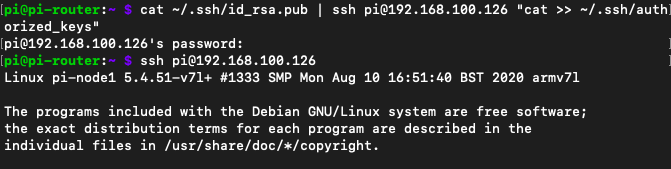
\includegraphics[width=\textwidth]{images/ssh-no-password.png}
    
    \item Repeat the above commands from each node, replacing the IP addresses each time with those of the other nodes in the cluster.
\end{itemize}

\section{Benchmark the Raspberry Pi cluster}

At this point, all necessary software has been installed on the cluster and the only thing remaining is to run the benchmark program \texttt{xhpl}. The task of distributing the benchmark workload across the cluster will be done by the \texttt{mpiexec} program, which was installed with MPICH.

\subsection{Create a hostfile}

In order for \texttt{mpiexec} to run tasks concurrently on the cluster, it needs to know the locations of each node on the cluster network, which is given by the node's IP address. The IP addresses will be written to a \emph{hostfile}, with one IP address per line. The hostfile will be passed to \texttt{mpiexec} through a command line argument. 

\begin{itemize}
    \item Navigate to the directory with the \texttt{xhpl} benchmarking program with the command \texttt{cd \tttilde/hpl-2.3/bin/rpi}.
    
    \item Run \texttt{nano hostfile-all.txt} to start editing a hostfile that will tell \texttt{mpiexec} to use every node on the cluster.
    
    For example, if the non-router nodes had IP addresses \texttt{192.168.100.43} and \texttt{192.168.100.126}, \texttt{hostfile-all.txt} should look like the following screenshot (where the \texttt{cat} command is being used to display the contents of the file in the terminal):
    
    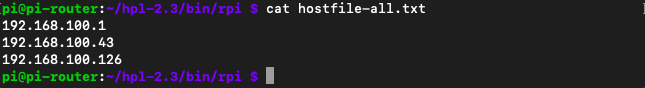
\includegraphics[width=\textwidth]{images/hostfile-all.png}
    
    \item Run the following command to test both the \texttt{hostfile-all.txt} hostfile and the cluster network:
\begin{verbatim}
mpiexec -hostfile hostfile-all.txt hostname
\end{verbatim}
    This executes the \texttt{hostname} command (which prints the current hostname) on each of the nodes designated by the hostfile. 
    
    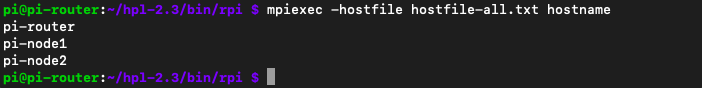
\includegraphics[width=\textwidth]{images/mpiexec-hostname.png}
    
    \item The \texttt{-n} argument can be used with \texttt{mpiexec} to set the number of \emph{tasks} (processes) assigned to the parallel job. Using the same hostfile, try different amounts of tasks to see how \texttt{mpiexec} automatically load-balances the tasks across the cluster. For example, with $12$ tasks assigned, \texttt{mpiexec} assigns $4$ to each of the $3$ nodes:
    
    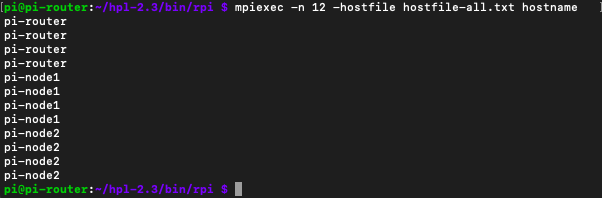
\includegraphics[width=\textwidth]{images/hostfile-all-tasks.png}
\end{itemize}

\subsection{Create an HPL tuning file}

The \texttt{xhpl} benchmark uses a file named \texttt{HPL.dat} to configure how large of a problem to solve and how the work should be distributed. A sample \texttt{HPL.dat} can be found in the same directory that \texttt{xhpl} was installed to, but for our purposes a new file will need to be generated from scratch. Since the structure of \texttt{HPL.dat} is quite complex, the following website exists to generate an \texttt{HPL.dat} file according to a few simple parameters:
\\~\\
\url{https://www.advancedclustering.com/act\_kb/tune-hpl-dat-file/}
\\~\\

The "Memory per Node" field controls both the memory used by the benchmark on each node and the size of the problem the benchmark solves. Even though a larger problem will take longer to complete than a smaller problem, if the larger problem uses the system's memory more efficiently then it may yield higher FLOPS, or floating-point operations per second, which is a standard way of measuring computing performance.

\begin{itemize}
    \item Use the above website to create an \texttt{HPL.dat} file with $3$ nodes, $1$ core per node, $1600$ MB of memory per node. Keep the default block size of $192$.
    
    \texttt{Note:} Even though each Raspberry Pi 4B node has four cores, an interaction between \texttt{mpiexec} and \texttt{xhpl} forces us to select $1$ core per node on the generator website. See the issues section for more details.
    
    \item If you haven't already, run the command \texttt{cd \tttilde/hpl-2.3/bin/rpi} to move to the directory containing \texttt{xhpl}.
    
    \item Run \texttt{rm HPL.dat} to remove the default \texttt{HPL.dat} file that was created when HPL was installed.
    
    \item Run \texttt{nano HPL.dat} and copy-paste the generated output from the website into the text editor. Save and close the file.
    
    \textbf{Note:} pasting into the terminal may require unusual input. On the MacOS default terminal, Command+V should work. On Windows terminals, right-clicking the terminal window should give an option to paste.
\end{itemize}

\subsection{Run the HPL benchmark}

\begin{itemize}
    \item Before running \texttt{xhpl}, make sure that its directory has the \texttt{hostfile-all.txt} and \texttt{HPL.dat} files created in the previous sections:
    
    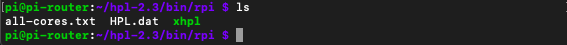
\includegraphics[width=\textwidth]{images/bin-before-xhpl.png}

    \item From the \texttt{\tttilde/hpl-2.3/bin/rpi} directory, use the following command to run the HPL benchmark (it's written as two lines here, but enter it as a single command on one line):
    
\begin{verbatim}
mpiexec -env LD_LIBRARY_PATH "/home/pi/openblas-install/lib"
  -hostfile all-cores.txt ./xhpl    
\end{verbatim}

    The \texttt{-env} argument is setting an environment variable on the remote nodes, and is necessary to tell remote nodes the location of their copies of OpenBLAS.
    
    \item When it begins running, HPL will list information about the benchmark parameters being used. If all Pis are working correctly on the problem, all of their fans should start making a fair amount of noise.
    
    \item While the benchmark is running, you can still SSH into any of the nodes on a different terminal window. Try using the following command on one or all of the nodes, which gives a live reading of its current temperature:
\begin{verbatim}
watch vcgencmd measure_temp
\end{verbatim}

    \item You can use the command \texttt{htop} to monitor the CPU usage on one or more of the nodes. While the benchmark is running, the usage of all $4$ cores of each node should be at or near $100$\%. 
    
    \textbf{Note:} You can use the F4 key in \texttt{htop} to filter the process list by name. While running the benchmark, filtering for \texttt{xhpl} will show only those benchmarking processes.

    \item After about $5$ minutes, the benchmark should conclude with a message similar to the following:
    
    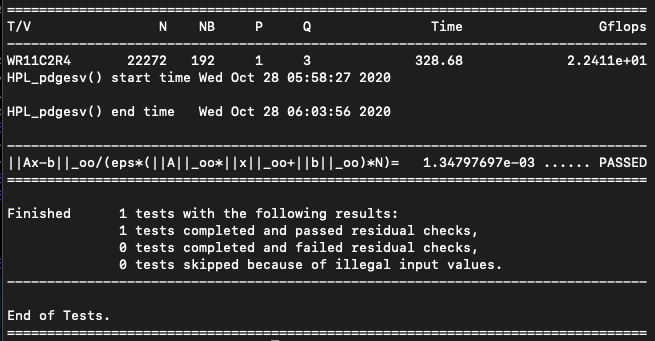
\includegraphics[width=\textwidth]{images/hpl-results.png}
    
    \item The primary measurement of interest is the \texttt{Gflops} of the benchmark, which is \texttt{2.2411e+01} in the above screenshot. This means that the cluster executed $22.411$ billion floating-point operations per second when all $3$ nodes were used.
    
    Also note the value of \texttt{N = 22272}, which is the size of the problem solved by the benchmark. This is one of the values in the \texttt{HPL.dat} file that is generated by the above website. The value of \texttt{N} will always be the same for the same generator inputs.
    
    \item Record your values of \texttt{N}, \texttt{Time}, and \texttt{Gflops} for the $3$-node cluster. Compare your results with the sample results given in Table \ref{tab:hpl-gflops} for the 3-node cluster. The time and Gflops will vary between trials, but your results should be within 20\% of the sample.
\end{itemize}

% Please add the following required packages to your document preamble:
% \usepackage{booktabs}
\begin{table}[h]
\centering
\begin{tabular}{@{}c|ccc@{}}
\toprule
\textbf{Nodes} & \textbf{N} & \textbf{Time (s)} & \textbf{Gflops} \\ \midrule
1              & 12,672     & 157.83            & 8.5966          \\
2              & 18,048     & 252.59            & 15.518          \\
3              & 22,272     & 328.68            & 22.411          \\ \bottomrule
\end{tabular}
\caption{Sample performance values for clusters of varying sizes.}
\label{tab:hpl-gflops}
\end{table}
    
\subsection{Benchmark a scaled-down cluster}

\begin{itemize}
    \item Use the same website as above to generate an \texttt{HPL.dat} file that uses $2$ nodes, $1$ core per node, $1600$ MB of memory, and a block size of $192$. Replace the previous \texttt{HPL.dat} file with the new configuration.
    
    \item The following command will now benchmark the $2$-node cluster:
\begin{verbatim}
mpiexec -env LD_LIBRARY_PATH "/home/pi/openblas-install/lib"
  -hostfile hostfile-all.txt ./xhpl
\end{verbatim}

    \textbf{Note:} Even though \texttt{hostfile-all.txt} still lists all $3$ nodes in the cluster, the \texttt{xhpl} program will only request two of them.  \texttt{mpiexec} will use the first two listed in the hostfile. Hence the same hostfile can be used, and the same command can be used to benchmark a cluster with less nodes.
    
    \item Record your values of \texttt{N}, \texttt{Time}, and \texttt{Gflops} for the $2$-node cluster. Compare your results to Table \ref{tab:hpl-gflops}. You should yield a \texttt{Gflops} value that is slightly more than $2/3$ the value from the $3$-node cluster.
    
    \item Repeat the above steps to benchmark a $1$-node "cluster" (use $1$ node in the website generator instead of $2$, generate a new \texttt{HPL.dat}, and replace the existing \texttt{HPL.dat}).
    
    \item Record your values of \texttt{N}, \texttt{Time}, and \texttt{Gflops} for the $1$-node "cluster". Again compare your results to Table \ref{tab:hpl-gflops}. You should yield a \texttt{Gflops} value that is slightly more than $1/3$ the value from the $3$-node cluster.
\end{itemize}

\section{Resources}
\begin{itemize}
    \item Official documentation for \texttt{mpiexec} in MPICH v3.3:
    
    \url{https://www.mpich.org/static/docs/v3.3/www1/mpiexec.html}
    
    \resource{resources/mpiexec.pdf}
    
    \textbf{Note:} There are other implementations of \texttt{mpiexec} in different MPI libraries with different documentations, but only the library MPICH is used in this lab.
    
    \item Official documentation for HPL:
    
    \url{https://www.netlib.org/benchmark/hpl/}
    
    \item Official documentation for the \texttt{HPL.dat} tuning file:
    
    \url{https://www.netlib.org/benchmark/hpl/tuning.html}
    
    \resource{resources/HPL\_Tuning.pdf}
    
    \item Generator for \texttt{HPL.dat} files:
    
    \url{https://www.advancedclustering.com/act_kb/tune-hpl-dat-file/}
    
    \item OpenBLAS FAQ:
    
    \url{https://github.com/xianyi/OpenBLAS/wiki/faq}
    
    \resource{resources/OpenBLAS\_FAQ.pdf}
\end{itemize}

\section{Known issues}

\subsection{Quantity of \texttt{xhpl} processes}

The expected behavior of \texttt{xhpl} is that the number of processes it uses corresponds to certain values in \texttt{HPL.dat}. Specifically, the integer values \texttt{P} and \texttt{Q}, which are set in the \texttt{HPL.dat} tuning file, should correspond to "number of processes used per node" and "number of nodes", respectively. In this way, the total number of processes used by \texttt{xhpl} across the entire cluster should be \texttt{P * Q}.

However, the observed behavior is that \texttt{4 * P * Q} processes are used instead. More precisely, varying the value of \texttt{Q} works as expected, controlling the number of nodes, but values of \texttt{P} seem to have $4$ times higher of an effect on the process count than described above: setting \texttt{P = 1} yields \texttt{4 * P * Q} processes on the cluster, \texttt{P = 2} yields \texttt{8 * P * Q} processes on the cluster, etc.

Since each node has $4$ cores, a \texttt{Q}-node cluster has \texttt{4 * Q} cores, and hence setting \texttt{P = 1} uses all cores on each node and results in ideal cluster performance. Using values of \texttt{P > 1} spawns more processes per node than there are cores, resulting in a much lower performance. 

It's very unlikely that this is a bug in either \texttt{mpiexec} or \texttt{xhpl}, since the value \texttt{P = 1} does yield optimal cluster performance. It's possible that when building HPL from source, HPL recognizes that there are $4$ cores on the node and defaults to creating $4$ processes to best fit those cores. This may be possible to change when building HPL.

\end{document}
